\documentclass[aspectratio=169,11pt]{beamer}

% Modern, editable Beamer deck based on TelcoCustomer.ipynb
% Compile with: pdflatex presentation.tex (twice for navigation)
% Keep the figures/ folder next to this file.

\usetheme{default}
\usepackage[utf8]{inputenc}
\usepackage[T1]{fontenc}
\usepackage[ngerman]{babel}
\usepackage{graphicx}
\usepackage{booktabs}
\usepackage{amsmath}
\usepackage{ragged2e}
\usepackage{lmodern}
\usepackage{microtype}
\usepackage{xcolor}
\usepackage{tikz}
\usetikzlibrary{arrows.meta}
\usetikzlibrary{shadows}

% --- Visual identity: midnight navy + electric cyan + violet ---
\definecolor{Midnight}{HTML}{10152B}
\definecolor{Navy}{HTML}{18213F}
\definecolor{Cyan}{HTML}{35D7E8}
\definecolor{Violet}{HTML}{8B7CFF}
\definecolor{Ink}{HTML}{202944}
\definecolor{Muted}{HTML}{69738B}
\definecolor{Paper}{HTML}{F5F7FC}
\definecolor{Line}{HTML}{DDE4F0}
\definecolor{SoftCyan}{HTML}{E5FAFC}
\definecolor{SoftViolet}{HTML}{F0EEFF}

\setbeamercolor{normal text}{fg=Ink,bg=Paper}
\setbeamercolor{structure}{fg=Cyan}
\setbeamercolor{frametitle}{fg=Midnight,bg=Paper}
\setbeamercolor{title}{fg=white}
\setbeamercolor{subtitle}{fg=Cyan}
\setbeamercolor{author}{fg=white}
\setbeamercolor{institute}{fg=white}
\setbeamercolor{date}{fg=white}
\setbeamercolor{itemize item}{fg=Cyan}
\setbeamercolor{itemize subitem}{fg=Violet}
\setbeamercolor{enumerate item}{fg=Midnight,bg=Cyan}
\setbeamercolor{block title}{fg=white,bg=Navy}
\setbeamercolor{block body}{fg=Ink,bg=white}
\setbeamercolor{caption name}{fg=Violet}

\setbeamertemplate{navigation symbols}{}
\setbeamertemplate{itemize item}{\raise0.2ex\hbox{\color{Cyan}\scriptsize$\blacklozenge$}}
\setbeamertemplate{itemize subitem}{\raise0.2ex\hbox{\color{Violet}\tiny$\bullet$}}
\setbeamertemplate{enumerate item}{\colorbox{Cyan}{\color{Midnight}\strut\insertenumlabel}}
\setbeamersize{text margin left=0.8cm,text margin right=0.8cm}

% Clean title bar and progress-style footer
\setbeamertemplate{frametitle}{
  \vspace{0.18cm}
  \begin{beamercolorbox}[wd=\paperwidth,ht=0.68cm,dp=0.15cm,leftskip=0.8cm,rightskip=0.8cm]{frametitle}
    \usebeamerfont{frametitle}\insertframetitle
  \end{beamercolorbox}
   {\color{Cyan}\rule{1.0cm}{1.0pt}}\hspace{0.3cm}{\color{Violet}\rule{13.0cm}{1.0pt}}
  }
\setbeamertemplate{footline}{%
  \leavevmode%
   {\hspace{0.5cm}\color{Cyan}\rule{1.0cm}{1.0pt}}\hspace{0.3cm}{\color{Violet}\rule{13.0cm}{1.0pt}}
  \hbox{% 
    \begin{beamercolorbox}[wd=.3\paperwidth,ht=2.5ex,dp=1.2ex,left]{footline}
      {\color{Muted}\scriptsize \hspace{0.5cm}TELCO CUSTOMER CHURN}
    \end{beamercolorbox}%
      \begin{beamercolorbox}[wd=.3\paperwidth,ht=2.5ex,dp=1.2ex,center]{footline}
      {\color{Muted}\insertframenumber\,/\,\inserttotalframenumber}
    \end{beamercolorbox}%
    \begin{beamercolorbox}[wd=.3\paperwidth,ht=2.5ex,dp=1.2ex,right]{footline}
      {\color{Muted}Analyse \& Modellierung}
    \end{beamercolorbox}%
  }%
  \vskip2pt%
}

\setbeamerfont{title}{series=\bfseries,size=\LARGE}
\setbeamerfont{subtitle}{size=\large}
\setbeamerfont{frametitle}{series=\bfseries,size=\Large}
\setbeamerfont{normal text}{size=\small}
\setlength{\parskip}{0.25em}

\title[Telco Customer Churn]{Analyse und Vorhersage von Kundenabwanderung}
\subtitle{Explorative Merkmalsanalyse und logistische Regression}
\author{A. Ebrahimi, H. Abdo}
\institute{BBQ - Online / PCED - 101}
\date{\today}

\begin{document}

%. ===============================================
\begin{frame}[plain]
\setbeamercolor{background canvas}{bg=Midnight}
%
\begin{tikzpicture}[remember picture,overlay]
\def\s{0.75}   % one scale factor for everything: 1 = original size
  % everything is anchored at the square's top-right corner and scaled together
  \begin{scope}[shift={([xshift=-0.25cm,yshift=-0.25cm]current page.north east)},
                scale=\s]

    % Navy square (3.5 x 3.5)
    \fill[Navy] (0,0) rectangle (-3.5,-3.5);

    % two lines below the square (centered under it)
    \draw[Cyan,opacity=0.55,line width={1*\s pt}]   (-3.25,-3.75) -- (-0.25,-3.75);
    \draw[Violet,opacity=0.75,line width={1*\s pt}] (-2.75,-3.95) -- (-0.75,-3.95);

    % circle figure, centered in the square
    \begin{scope}[shift={(-1.75,-1.75)}]

      \fill[Violet] (0,0) circle (0.75cm);
      \fill[Cyan,opacity=0.18] (0,0) circle (1.5cm);

      \draw[Navy, line width={1.5*\s pt}, dotted] (-0.75,0) -- (0.75,0);
      \draw[Navy, line width={1.5*\s pt}, dotted] (0,0.75) -- (0,-0.75);

      \foreach \a in {45,-45,-135,-225}{
        \begin{scope}[rotate=\a, opacity=0.9]
          \shade[shading=axis, shading angle=90,
                 left color=Cyan!65!black, right color=Cyan!15!black,
                 middle color=Cyan!40!white]
            (-0.11,-1.5) rectangle (0.11,-0.27);
          \fill[Cyan!70!black] (-0.17,-0.3) -- (0,0) -- (0,-0.3) -- cycle;
          \fill[Cyan!45!white] (0.17,-0.3) -- (0,0) -- (0,-0.3) -- cycle;
          \fill[Cyan!80!black] (-0.17,-0.3) -- (0.17,-0.3) -- (0.11,-0.27) -- (-0.11,-0.27) -- cycle;
        \end{scope}
      }
    \end{scope}
  \end{scope}
\end{tikzpicture}
  {\vspace{0.1cm} 
  
  \color{Cyan}\small DATA SCIENCE \hspace{0.4em}/\hspace{0.4em} CUSTOMER ANALYTICS}
  \vspace{0.1cm}
    \begin{center}
  {\color{Violet}\bfseries\fontsize{22}{28}\selectfont Analyse und Vorhersage\\ von Kundenabwanderung}
  \end{center} 
  \vspace{0.50cm}
    \begin{center} {\color{Cyan}\large Explorative Merkmalsanalyse und logistische Regression} \end{center}

  \vspace{0.5cm}
 \begin{center} {\color{Navy}\normalsize \insertauthor} \end{center}

  \vspace{0.25cm}
  \begin{center} \color{Violet}\small \insertinstitute \end{center}
    \vspace{0.50cm}
  \begin{center} \insertdate \end{center}
  \vfill
   {\color{Cyan}\rule{1.0cm}{1.0pt}}\hspace{0.3cm}{\color{Violet}\rule{13.0cm}{1.0pt}}
  \vspace{0.35cm}
\end{frame}
%. ===============================================
\begin{frame}{Überblick}

  \uncover<1->{%
  \begin{beamercolorbox}[rounded=true,sep=0.15cm,wd=\linewidth]{block body}
    {\color{Cyan}\large\bfseries 01 \hspace{0.3em} \color{Violet}\large\bfseries THEMA}

    \vspace{0.10cm}
    \uncover<2->{\textbf{Kundenabwanderung (Churn)} bei einem Telekommunikationsanbieter.}
  \end{beamercolorbox}}

  \vfill

  \uncover<3->{%
  \begin{beamercolorbox}[rounded=true,sep=0.15cm,wd=\linewidth]{block body}
    {\color{Cyan}\large\bfseries 02 \hspace{0.3em} \color{Violet}\large\bfseries ZIEL}

    \vspace{0.1cm}
    \uncover<4->{Zusammenhänge untersuchen und ein erstes Vorhersagemodell aufbauen.}
  \end{beamercolorbox}}

  \vfill

  \uncover<5->{%
  \begin{beamercolorbox}[rounded=true,sep=0.15cm,wd=\linewidth]{block body}
    {\color{Cyan}\large\bfseries 03 \hspace{0.3em} \color{Violet}\large\bfseries DATEN}

    \vspace{0.1cm}
    \uncover<6->{%
      IBM Telco Customer Churn:
      \hspace{0.1cm}
      {\color{Midnight}\bfseries\selectfont 7\,043}
      {\color{Muted}\small Datensätze \hspace{0.4em}\textbullet\hspace{0.4em} {\bfseries\selectfont 21} Spalten}}
  \end{beamercolorbox}}

  \vfill

  \uncover<7->{%
  \begin{beamercolorbox}[rounded=true,sep=0.15cm,wd=\linewidth]{block body}
    {\color{Cyan}\large\bfseries 04 \hspace{0.3em} \color{Violet}\large\bfseries VORGEHEN}

    \vspace{0.10cm}
    \uncover<8->{Bereinigung, Feature-Analyse, Kodierung und logistische Regression.}
  \end{beamercolorbox}}

\end{frame}
%. ===============================================
\begin{frame}{Fragestellung und Zielvariable}
  \begin{itemize}
    \item<1-> Zielvariable ist \texttt{Churn}: Kündigung = 1, keine Kündigung = 0.\\[0.3cm]
    \item<2-> Es werden Kunden-, Vertrags- und Dienstleistungsmerkmale betrachtet.\\[0.3cm]
    \item<3-> Der Churn-Anteil nach der Bereinigung beträgt rund 26{,}6\,\%; etwa 73{,}4\,\% bleiben.\\[0.3cm]
    \item<4-> Die Analyse soll relevante Merkmale sichtbar machen und die Vorhersage auf unbekannten Daten prüfen.
  \end{itemize}
\end{frame}
%. ===============================================
\begin{frame}{Strategie / Analysepipeline}
  \begin{enumerate}
    \item<1->~ {\onslide<2-> Datensatz laden und Duplikate bzw. fehlende Werte prüfen.}\\[0.05cm]
    \item<3->~ {\onslide<4-> Identifikator \texttt{customerID} entfernen und \texttt{TotalCharges} numerisch konvertieren.}\\[0.05cm]
    \item<5->~ {\onslide<6-> Merkmale explorativ vergleichen: Spannweite der Churn-Raten, Chi-Quadrat-Test und Phi-Koeffizient.}\\[0.05cm]
    \item<7->~ {\onslide<8-> Merkmale auswählen und kategoriale Variablen kodieren (One-Hot-Encoding).}\\[0.05cm]
    \item<9->~ {\onslide<10-> Daten stratifiziert in Training (80\,\%) und Test (20\,\%) teilen.}\\[0.05cm]
    \item<11->~ {\onslide<12-> Numerische Merkmale skalieren und logistische Regression trainieren.}\\[0.05cm]
    \item<13->~ {\onslide<14-> Güte mit Accuracy, ROC-AUC, Konfusionsmatrix sowie Precision/Recall/F1 bewerten.}
  \end{enumerate}
\end{frame}
%. ===============================================
\begin{frame}{Datenaufbereitung}
  \begin{itemize}
    \item<1-> \textbf{Ausgangsdaten:}\uncover<2->{ 7\,043 Zeilen, 21 Spalten.}\\[0.3cm]
    \item<3->\textbf{Markmale Untersuchungen:} \uncover<4->{Nach Entfernung des Identifikators und Bereinigung: 7\,032 Zeilen; 11 nicht numerisch interpretierbare \texttt{TotalCharges}-Werte wurden zu fehlenden Werten und anschließend entfernt.}\\[0.3cm]
    \item<5->\textbf{Erklärende Merkmale:} \uncover<6->{\texttt{customerID:}wird nicht als erklärendes Merkmal verwendet.}\\[0.3cm]
    \item<7->\textbf{Encoding:} \uncover<8->{Kategoriale Merkmale werden numerisch kodiert; bei One-Hot-Encoding wird eine Referenzkategorie weggelassen}.\\[0.3cm]
    \item<9-> \textbf{Standardisierung:}\uncover<10->{Für die logistische Regression werden \texttt{tenure} und \texttt{MonthlyCharges} standardisiert.}
  \end{itemize}
\end{frame}
%. ===============================================
\begin{frame}{Strategie der Merkmalsanalyse}
  \begin{itemize}
    \item<1-> \textbf{Feature Screening:} \uncover<2->{Differenz zwischen höchster und niedrigster Churn-Rate je Merkmal.}\\[0.3cm]
    \item<3-> \textbf{Chi-Quadrat-Test:} \uncover<4->{Prüft, ob kategoriale Merkmale und Churn statistisch zusammenhängen.}\\[0.3cm]
    \item<5-> \textbf{Phi-Koeffizient:}\uncover<6->{ Beschreibt die Stärke des Zusammenhangs für geeignete binäre Variablen.}\\[0.3cm]
    \item<7-> \textbf{Signifikanzniveau:} \uncover<8->{Wir haben  das Signifikanzniveau von $\alpha=0{,}01$ verwendet.}\\[0.3cm]
    \item<9-> \textbf{Interpretation mit Vorsicht:} \uncover<10->{\texttt{MonthlyCharges} benötigt besondere Aufmerksamkeit; Zusammenhang bedeutet nicht automatisch Kausalität.}
  \end{itemize}
\end{frame}
%. ===============================================
\begin{frame}{Explorative Analyse}
  \centering
  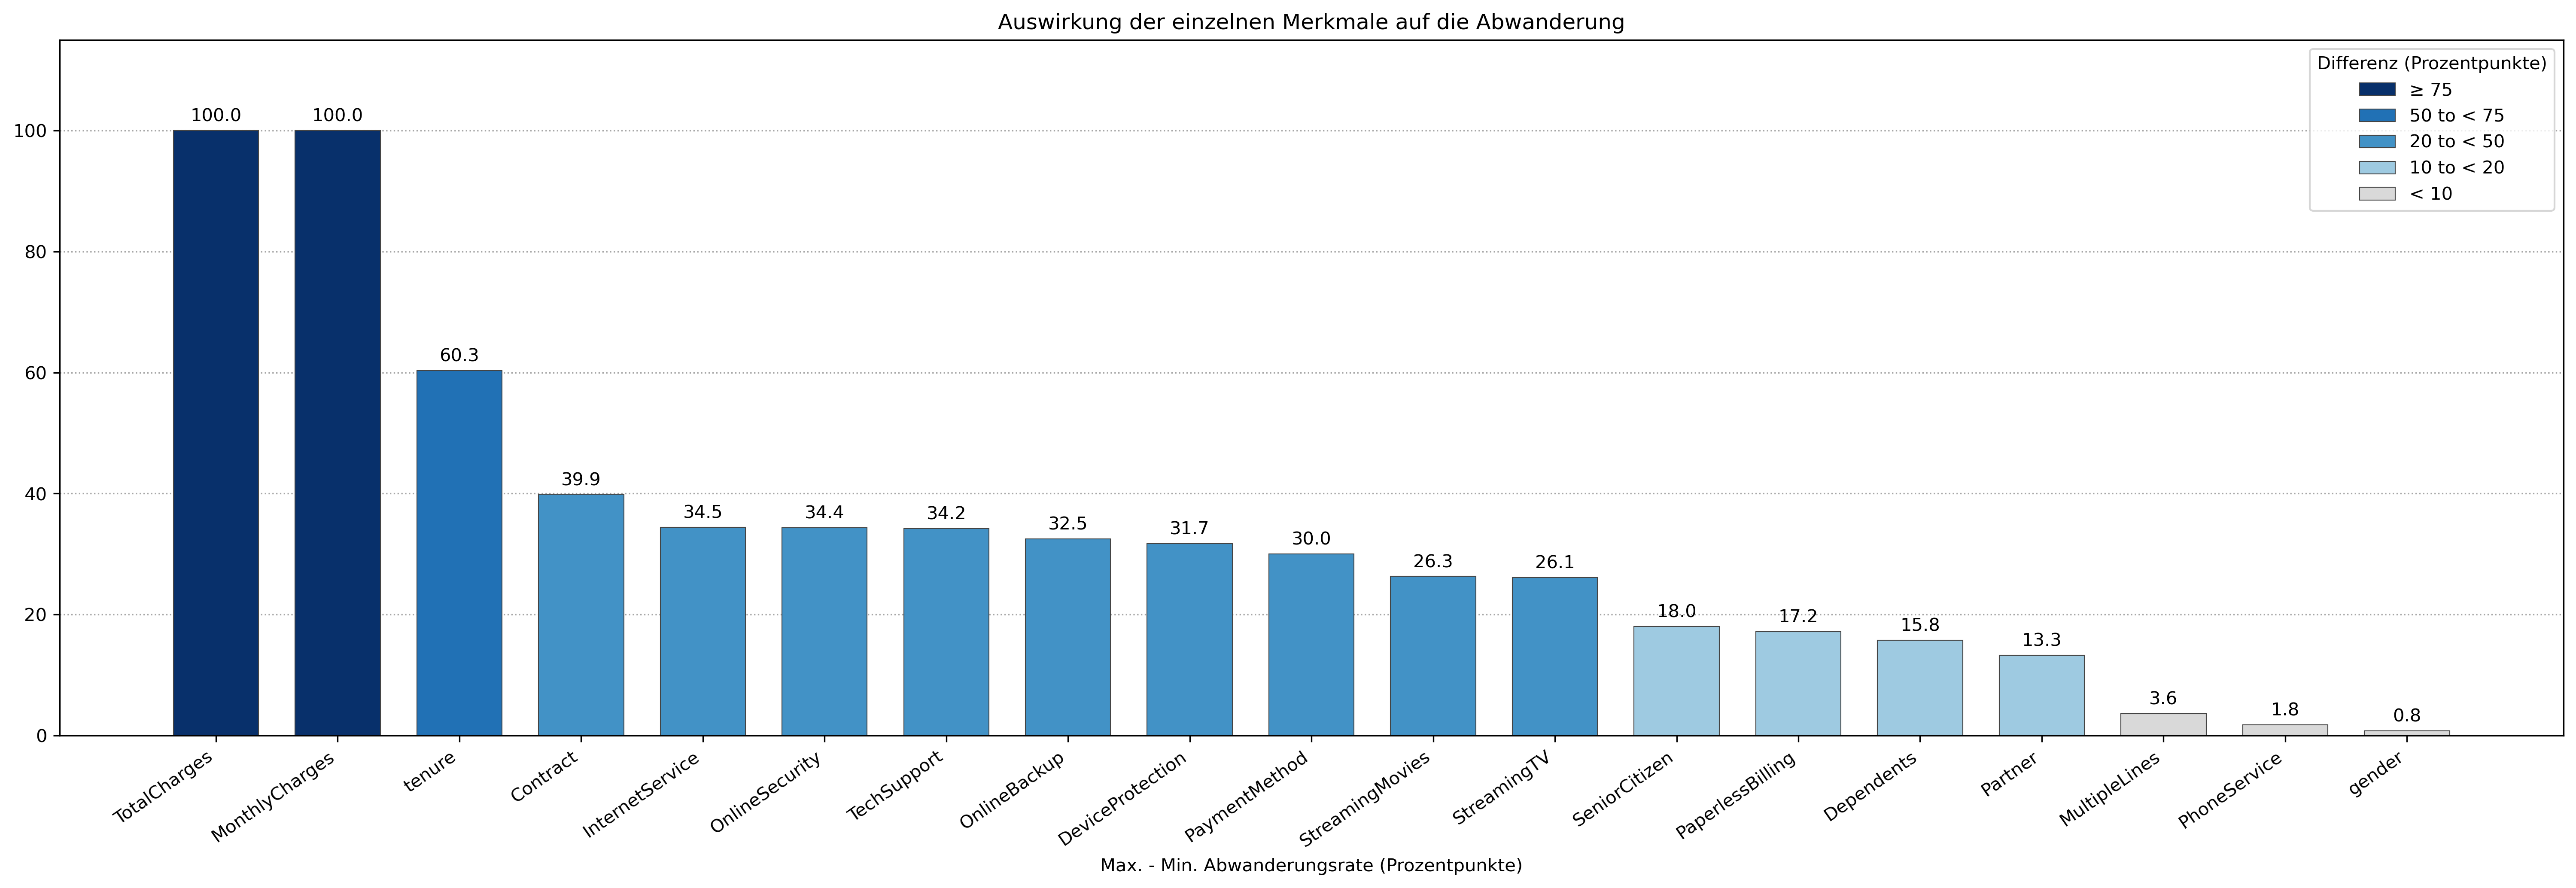
\includegraphics[width=0.92\textwidth,height=0.72\textheight,keepaspectratio]{figures/effect_features_on_churn_group.png}

  \vspace{0.12cm}
  \uncover<2->{{\color{Muted}\scriptsize Unterschiede der Churn-Raten nach Merkmalen}}
\end{frame}

\begin{frame}{Zusammenhang zwischen Merkmalen und Churn}
  \centering
  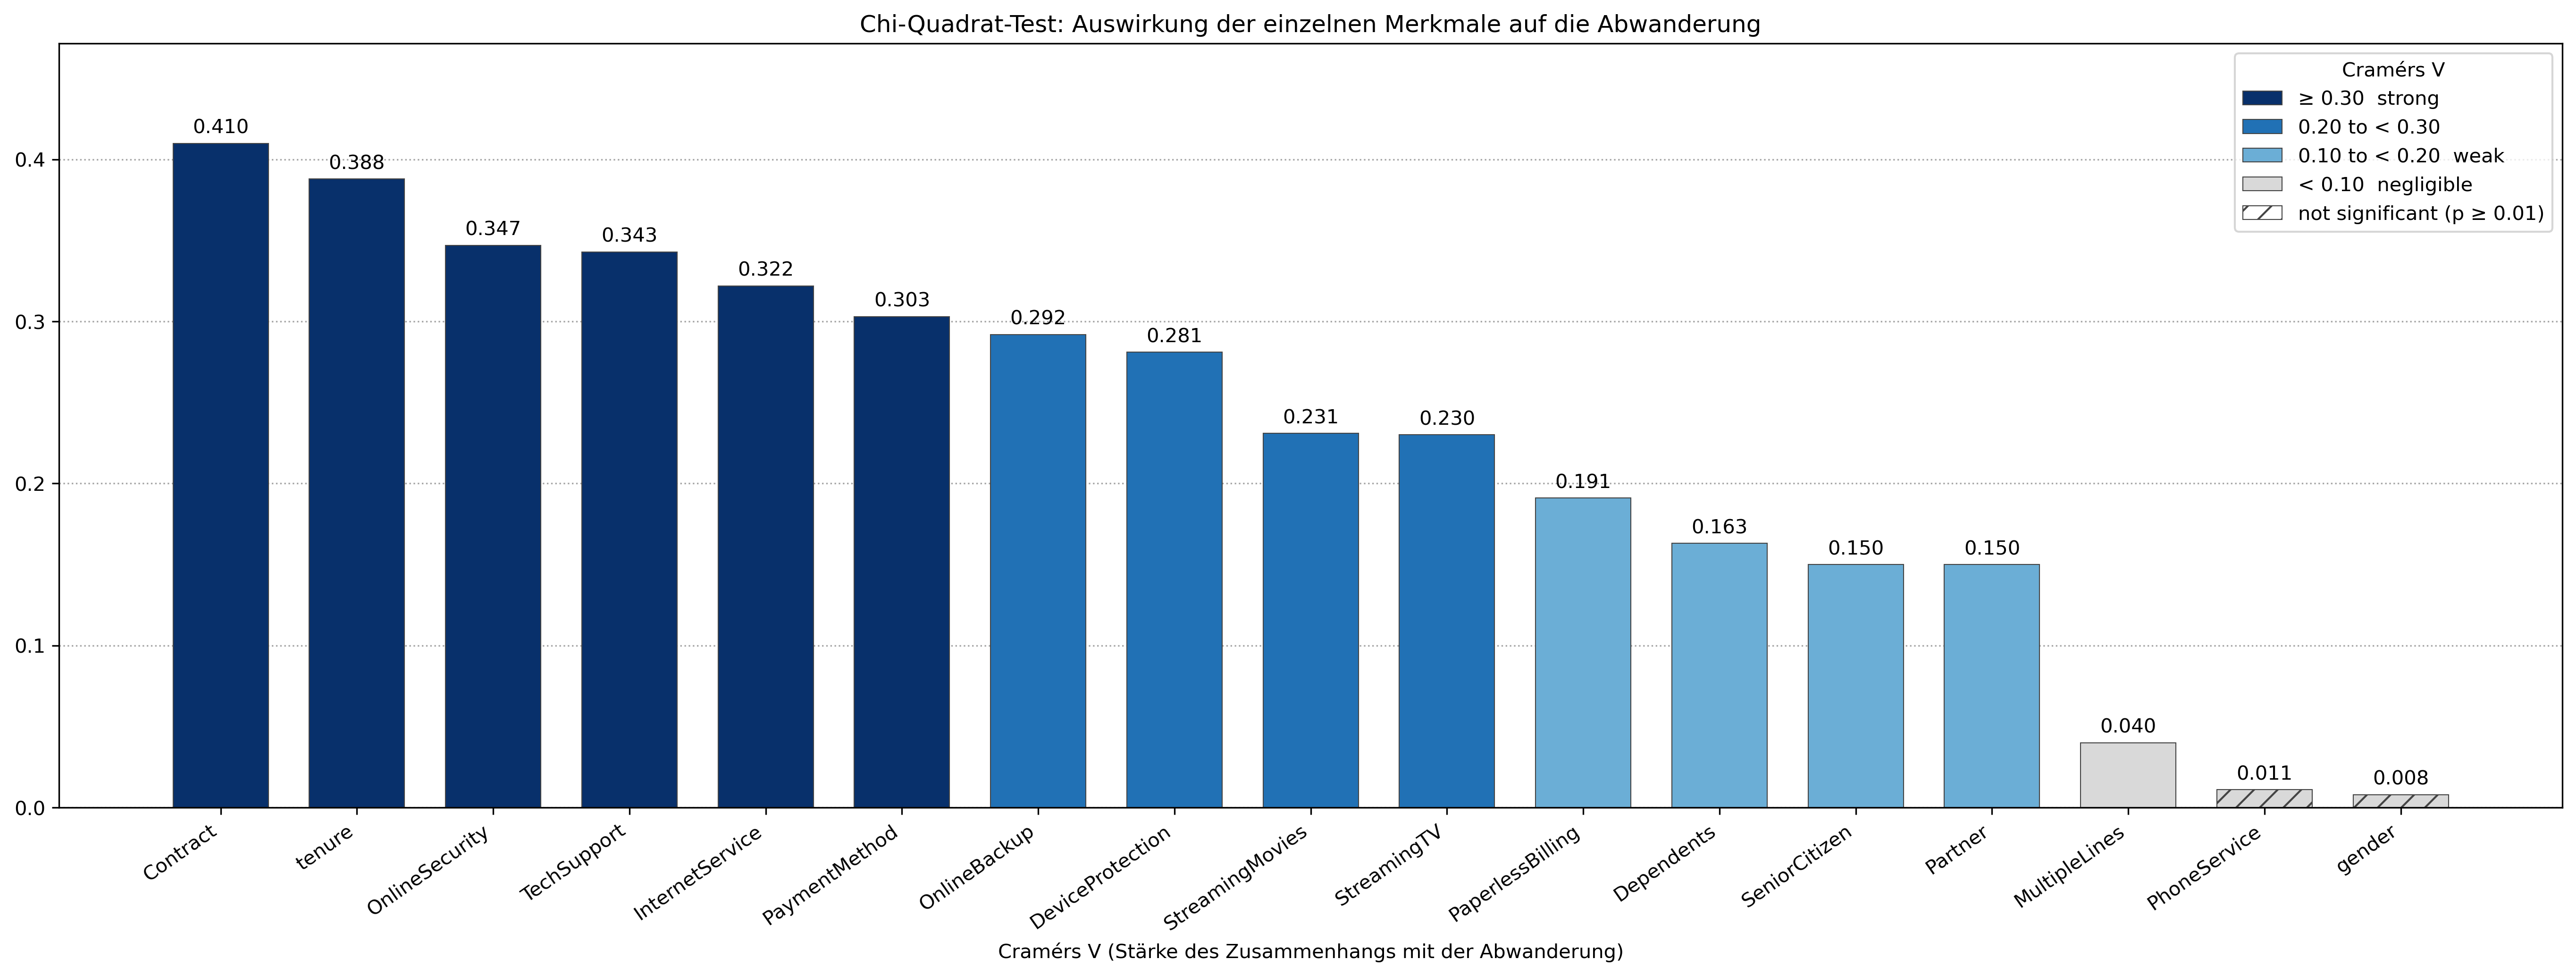
\includegraphics[width=0.92\textwidth,height=0.72\textheight,keepaspectratio]{figures/effect_features_on_churn_chi2.png}

  \vspace{0.12cm}
  \uncover<2->{{\color{Muted}\scriptsize Chi-Quadrat-Test und Phi-Koeffizient}}
\end{frame}
%. ===============================================

\begin{frame}{Zusammenfassung der Merkmalskombinationen}

  \uncover<1->{%
  \begin{beamercolorbox}[rounded=true,sep=0.15cm,wd=\linewidth]{block body}
    {\color{Cyan}\large\bfseries 01 \hspace{0.3em} CHURN-RATE}

    \vspace{0.10cm}
    \uncover<2->{Die zehn stärksten Kombinationen liegen zwischen
      {\color{Midnight}\bfseries 52{,}18\,\%} und {\color{Midnight}\bfseries 54{,}65\,\%}
      und damit rund doppelt so hoch wie der Durchschnitt von 26{,}6\,\%.}
  \end{beamercolorbox}}

  \vfill

  \uncover<3->{%
  \begin{beamercolorbox}[rounded=true,sep=0.15cm,wd=\linewidth]{block body}
    {\color{Violet}\large\bfseries 02 \hspace{0.3em} HÄUFIGE MERKMALE}

    \vspace{0.1cm}
    \uncover<4->{\texttt{PaymentMethod\_Electronic check} (6 von 10),
      \texttt{Contract\_Month-to-month} (4 von 10) und
      \texttt{SeniorCitizen} (3 von 10) kommen am häufigsten vor.}
  \end{beamercolorbox}}

  \vfill

  \uncover<5->{%
  \begin{beamercolorbox}[rounded=true,sep=0.15cm,wd=\linewidth]{block body}
    {\color{Cyan}\large\bfseries 03 \hspace{0.3em} EINORDNUNG}

    \vspace{0.1cm}
    \uncover<6->{Jede Kombination umfasst
      {\color{Midnight}\bfseries 375} Kunden. Die Zusammenhänge zeigen,
      welche Gruppen gefährdet sind, belegen aber keine Kausalität.}
  \end{beamercolorbox}}

\end{frame}

%. ===============================================
\begin{frame}{Merkmalskombinationen mit hoher Churn-Rate}
  \centering
  \footnotesize
  \renewcommand{\arraystretch}{1.05}
  \begin{tabular}{l l r r}
    \toprule
    {\color{Muted}\textbf{\#}} &
    {\color{Midnight}\textbf{Kombination von zwei Merkmalen}} &
    {\color{Midnight}\textbf{Kundenanzahl}} &
    {\color{Midnight}\textbf{Churn-Rate}} \\
    \midrule

    \visible<1->{\color{Cyan}\bfseries   1} &
    \visible<1->{SeniorCitizen mit Contract\_Month-to-month} &
    \visible<1->{807} &
    \visible<1->{\color{Cyan}\bfseries 54.65} \\
    \addlinespace[2pt]

    \visible<2->{\color{Violet}\bfseries 2} &
    \visible<2->{InternetService\_Fiber optic mit Contract\_Month-to-month} &
    \visible<2->{2128} &
    \visible<2->{\color{Violet}\bfseries 54.61} \\
    \addlinespace[2pt]

    \visible<3->{\color{Cyan}\bfseries   3} &
    \visible<3->{OnlineBackup\_No mit PaymentMethod\_Electronic check} &
    \visible<3->{1428} &
    \visible<3->{\color{Cyan}\bfseries 53.92} \\
    \addlinespace[2pt]

    \visible<4->{\color{Violet}\bfseries 4} &
    \visible<4->{Contract\_Month-to-month mit PaymentMethod\_Electronic check} &
    \visible<4->{1850} &
    \visible<4->{\color{Violet}\bfseries 53.73} \\
    \addlinespace[2pt]

    \visible<5->{\color{Cyan}\bfseries   5} &
    \visible<5->{SeniorCitizen mit PaymentMethod\_Electronic check} &
    \visible<5->{594} &
    \visible<5->{\color{Cyan}\bfseries 53.37} \\
    \addlinespace[2pt]

    \visible<6->{\color{Violet}\bfseries 6} &
    \visible<6->{InternetService\_Fiber optic mit PaymentMethod\_Electronic check} &
    \visible<6->{1595} &
    \visible<6->{\color{Violet}\bfseries 53.23} \\
    \addlinespace[2pt]

    \visible<7->{\color{Cyan}\bfseries   7} &
    \visible<7->{TechSupport\_No mit PaymentMethod\_Electronic check} &
    \visible<7->{1730} &
    \visible<7->{\color{Cyan}\bfseries 53.18} \\
    \addlinespace[2pt]

    \visible<8->{\color{Violet}\bfseries 8} &
    \visible<8->{OnlineSecurity\_No mit PaymentMethod\_Electronic check} &
    \visible<8->{1734} &
    \visible<8->{\color{Violet}\bfseries 53.17} \\
    \addlinespace[2pt]

    \visible<9->{\color{Cyan}\bfseries   9} &
    \visible<9->{SeniorCitizen mit OnlineBackup\_No} &
    \visible<9->{614} &
    \visible<9->{\color{Cyan}\bfseries 52.77} \\
    \addlinespace[2pt]

    \visible<10->{\color{Violet}\bfseries 10} &
    \visible<10->{MonthlyCharges mit Contract\_Month-to-month} &
    \visible<10->{870} &
    \visible<10->{\color{Violet}\bfseries 52.18} \\

    \bottomrule
  \end{tabular}

  \vspace{0.05cm}
  \visible<11->{
  \begin{beamercolorbox}[rounded=true,sep=-.40cm,wd=\linewidth]{block body}
    \small Diese Tabelle zeigt die höchste Churn-Rate aus der Kombination
    zweier Merkmale, die Anzahl der Kunden sowie die Churn-Rate.
  \end{beamercolorbox}}
\end{frame}
%. ===============================================
%. ===============================================
\begin{frame}{Modellaufbau}
  \begin{itemize}
    \item<1-> \textbf{Modell:} \uncover<2->{logistische Regression aus \texttt{scikit-learn}.}\\[0.5cm]

    \item<3-> \textbf{Aufteilung:} \uncover<4->{80\,\% Trainingsdaten und 20\,\% Testdaten, mit \texttt{stratify=y} und \texttt{random\_state=42}.}\\[0.5cm]

    \item<5-> \textbf{Trainingsdaten:} \uncover<6->{Die Vorverarbeitung wird anhand der Trainingsdaten angepasst; dieselbe Skalierung wird auf den Testdaten angewendet.}\\[0.5cm]

    \item<7-> \textbf{Was liefert das Modell:} \uncover<8->{Das Modell liefert sowohl Klassenprognosen als auch geschätzte Churn-Wahrscheinlichkeiten.}
  \end{itemize}
\end{frame}
%. ===============================================
\begin{frame}{Ergebnisse auf dem Testdatensatz}
  \begin{columns}[T,onlytextwidth]
    \column{0.32\textwidth}
      \uncover<1->{%
      \begin{beamercolorbox}[rounded=true,sep=0.32cm,wd=\linewidth]{block body}
        {\color{Muted}\scriptsize ACCURACY}
        \vspace{0.08cm}

        {\color{Midnight}\bfseries\fontsize{16}{16}\selectfont 78{,}75\,\%}
        \vspace{0.1cm}

        {\color{Cyan}\rule{0.85cm}{2pt}}
      \end{beamercolorbox}}
    \column{0.32\textwidth}
      \uncover<2->{%
      \begin{beamercolorbox}[rounded=true,sep=0.32cm,wd=\linewidth]{block body}
        {\color{Muted}\scriptsize ROC-AUC}
        \vspace{0.08cm}

        {\color{Midnight}\bfseries\fontsize{16}{16}\selectfont 0{,}830}
        \vspace{0.1cm}

        {\color{Violet}\rule{0.85cm}{2pt}}
      \end{beamercolorbox}}
    \column{0.32\textwidth}
      \uncover<3->{%
      \begin{beamercolorbox}[rounded=true,sep=0.32cm,wd=\linewidth]{block body}
        {\color{Muted}\scriptsize RECALL · CHURN}
        \vspace{0.08cm}

        {\color{Midnight}\bfseries\fontsize{16}{16}\selectfont 0{,}53}
        \vspace{0.1cm}

        {\color{Cyan}\rule{0.85cm}{2pt}}
      \end{beamercolorbox}}
  \end{columns}
  \vspace{0.35cm}
  \centering
  \uncover<4->{%
  \begin{tabular}{lr}
    \toprule
    \textbf{Metrik} & \textbf{Ergebnis} \\
    \midrule
    Precision (Churn = 1) & 0{,}62 \\
    F1-Score (Churn = 1) & 0{,}57 \\
    \bottomrule
  \end{tabular}}

  \vspace{0.2cm}
  \uncover<5->{%
  \begin{beamercolorbox}[rounded=true,sep=0.22cm,wd=\linewidth]{block body}
    \small Das Modell erkennt einen Teil der kündigenden Kunden, verpasst beim Schwellenwert 0{,}5 jedoch noch viele. Accuracy allein reicht daher nicht aus; Recall und Fehlklassifikationskosten sind ebenfalls wichtig.
  \end{beamercolorbox}}
\end{frame}
%. ===============================================
\begin{frame}{Konfusionsmatrix und Einordnung}
  \centering
  \uncover<1->{%
  \begin{tabular}{lrr}
    \toprule
    & \textbf{Prognose: bleibt} & \textbf{Prognose: kündigt} \\
    \midrule
    Tatsächlich: bleibt & 911 & 122 \\
    Tatsächlich: kündigt & 177 & 197 \\
    \bottomrule
  \end{tabular}}
  \vspace{0.8em}
  \begin{itemize}
    \item<2-> 197 von 374 tatsächlichen Kündigungen wurden erkannt.
    \item<3-> 177 Kündigungen wurden übersehen; eine mögliche nächste Verbesserung ist die Prüfung des Entscheidungsschwellenwerts.
    \item<4-> Im Notebook wird außerdem starke Multikollinearität bei einigen One-Hot-Spalten gemeldet. Das sollte vor einer Koeffizienteninterpretation geprüft werden.
  \end{itemize}
\end{frame}
%. ===============================================
\begin{frame}{Fazit und nächste Schritte}
  \uncover<1->{%
  \begin{beamercolorbox}[rounded=true,sep=0.35cm,wd=\linewidth]{block body}
    {\color{Cyan}\bfseries KERNAUSSAGE}
    
    \vspace{0.15cm}
    \uncover<2->{
    Die Pipeline liefert ein erstes brauchbares Basismodell: 78{,}7\,\% Accuracy und 0{,}83 ROC-AUC. Die Erkennung kündigender Kunden bleibt mit einem Recall von 0{,}53 ausbaufähig.}
  \end{beamercolorbox}}

  \vspace{0.15cm}
  \uncover<3->{{\color{Midnight}\bfseries Nächste Schritte}}
  \begin{itemize}
  \item<4->~ \uncover<5->{Multikollinearität reduzieren und Koeffizienten sorgfältig interpretieren.}\\[0.3cm]
    \item<6->~ \uncover<7->{Weitere Modelle vergleichen und Cross-Validation durchführen.}\\[0.3cm]
    \item<8->~ \uncover<9->{Entscheidungsschwellenwert an den Geschäftszielen und den Kosten von Fehlklassifikationen ausrichten.}
  \end{itemize}
\end{frame}
%. ===============================================
%. ===============================================
\begin{frame}{Vielen Dank}
  \vfill

  \uncover<1->{%
  \begin{beamercolorbox}[rounded=true,sep=0.35cm,wd=\linewidth,center]{block body}
    {\color{Cyan}\large\bfseries \hspace{0.3em} DANKE}

    \vspace{0.15cm}
    \uncover<2->{%
      {\color{Midnight}\bfseries\fontsize{16}{16}\selectfont Vielen Dank für Ihre Aufmerksamkeit!}

      \vspace{0.1cm}
      {\color{Cyan}\rule{0.85cm}{2pt}}}
  \end{beamercolorbox}}

  \vfill

  \uncover<3->{%
  \begin{beamercolorbox}[rounded=true,sep=0.35cm,wd=\linewidth,center]{block body}
    {\color{Violet}\large\bfseries \hspace{0.3em} FRAGEN}

    \vspace{0.15cm}
    \uncover<4->{%
      Gibt es Fragen oder Anmerkungen?

      \vspace{0.1cm}
      {\color{Violet}\rule{0.85cm}{2pt}}}
  \end{beamercolorbox}}

  \vfill
\end{frame}
%. ===============================================
\end{document}
